		\chapter{Биотический фон в сообществах {\it Macoma balthica}}

	\section{Белое море}
Описание сообществ макробентоса проводили на 6 мониторинговых участках в Кандалакшском заливе отдельно на каждом мареографическом уровне. 
Таким образом, всего было получено $12$ таксономических списков.
Всего на  исследованных участках было обнаружено $57$ таксонов беспозвоночных (приложение~\ref{app:species}, таблица~\ref{tab:White_species}).
Из них только непосредственно {\it Macoma balthica} встречена во всех 12 описаниях.
$18$ таксонов из $57$ были представлены только в одном описании.
Количество таксонов в одном описании колебалось от $5$ в верхнем горизонте материковой литорали в Лувеньге до $42$ у нуля глубин в Южной губе о.~Ряшкова.
По количеству таксонов преобладали представители Polychaeta (22 таксона).

%Классификация участков по видовому составу была проведена при помощи кластеризации методом ближайшего соседа по коэффициенту Жаккара. 
%Достоверность кластеров оценивали с помощью анализа сходства профилей (SIMPROF) (\cite{Clarke_et_al_2008}).

При анализе фаун с выделением горизонтов было выделено 6 групп участков ($p<0,05$) (рис.~\ref{ris:cluster_white_species_tidal}). 
	\begin{figure}[p]
		\begin{center}
			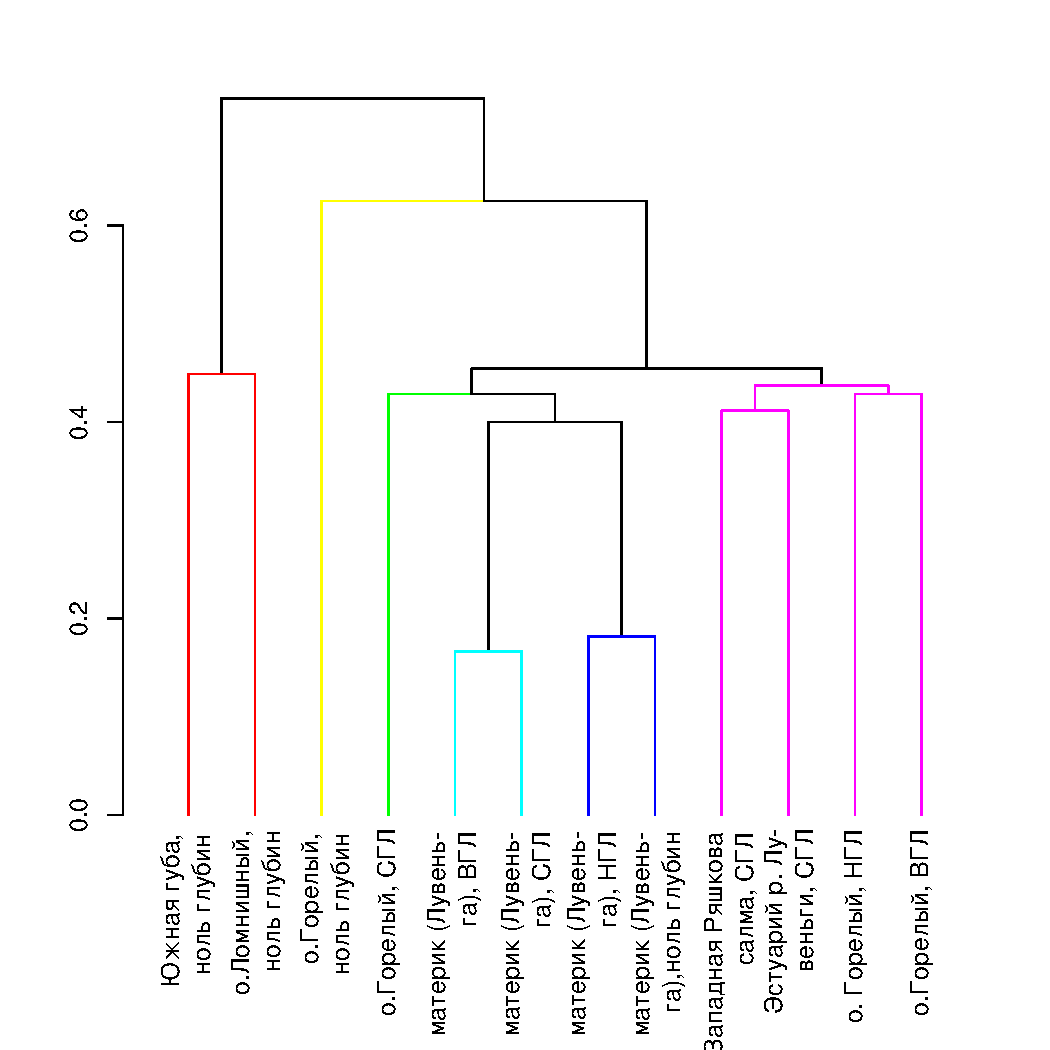
\includegraphics{../White_Sea/soobshestvo/White_fauna_tidal_jaccard_single_1.pdf}
		\end{center}
	\caption{Классификация отдельных горизонтов литорали в Белом море по видовому составу}
	\label{ris:cluster_white_species_tidal}

	\footnotesize{Кластеризация по методу ближайшего соседа с использованием коэффициента Жаккара. По оси ординат --- коэффициент Жаккара. Цветом показаны кластеры, достоверно выделяющиеся при 5\% уровне значимости.}
	\end{figure}
Группировка станций по кластерам неоднородна. 
Три кластера демонстрируют сходство по географическому признаку (голубой, синий и, отчасти, фиолетовый на рис.~\ref{ris:cluster_white_species_tidal}), три по мареографическому признаку (красный, синий и голубой кластер на рис.~\ref{ris:cluster_white_species_tidal}), остальные не показывают явной приуроченности.


При анализе фаун отдельных участков было выделено три группы (рис.~\ref{ris:cluster_white_species_sites}.) 
	\begin{figure}[p]
		\begin{center}
			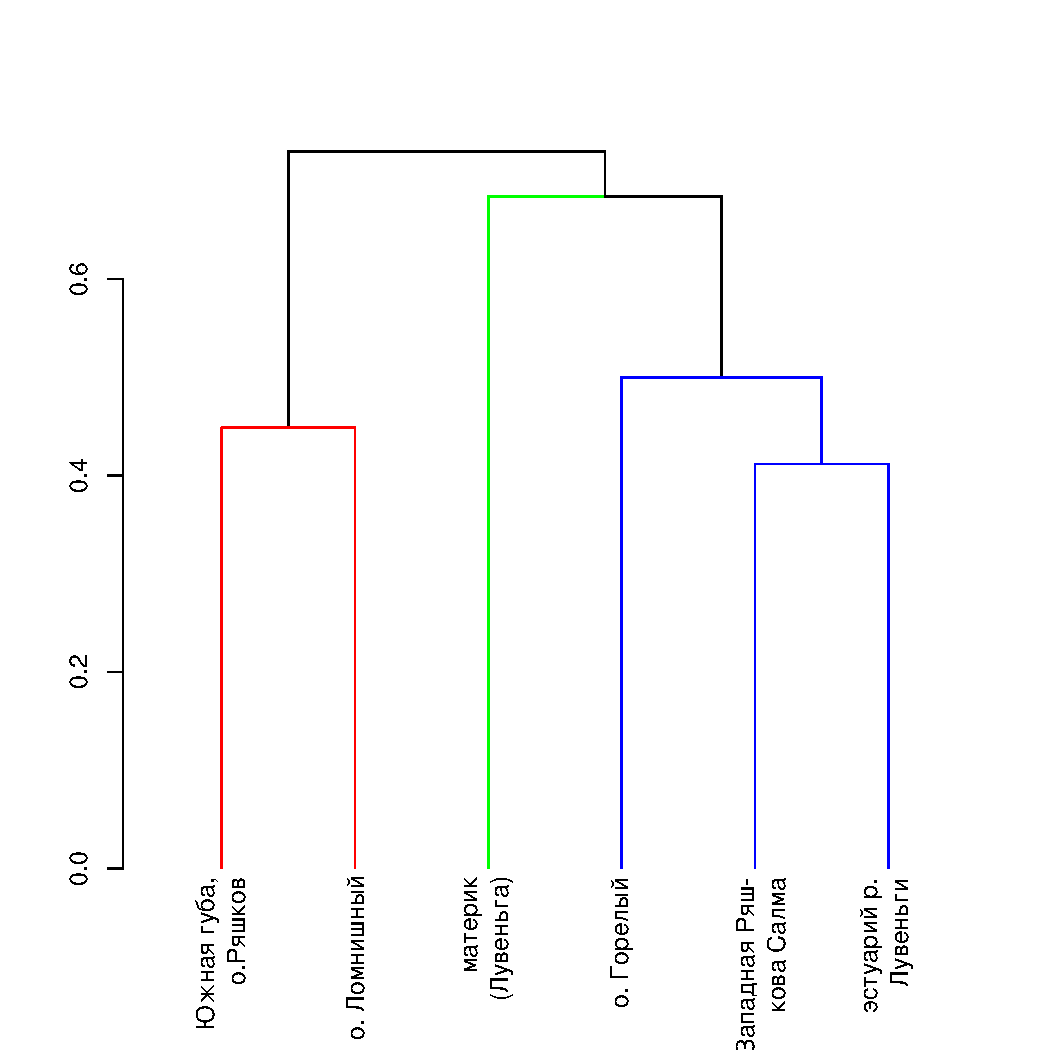
\includegraphics{../White_Sea/soobshestvo/White_fauna_sites_jaccard_single_1.pdf}
		\end{center}
	\caption{Классификация исследованных участков в Белом море по видовому составу}
	\label{ris:cluster_white_species_sites}

	\footnotesize{Кластеризация по методу ближайшего соседа с использованием коэффициента Жаккара. По оси ординат --- коэффициент Жаккара. Цветом показаны кластеры, достоверно выделяющиеся при 5\% уровне значимости.}
	\end{figure}
Первый кластер образуют сообщества в  Южной губе о.~Ряшкова и на о.~Ломнишный, которые близки как географически, так и мареографически (исследованы сообщества у нуля глубин).
В отдельный кластер попадает материковая литораль в районе Лувеньги, что связано, по-видимому, с максимальным биотопическим разнообразием на данном участке, поскольку здесь в пределах ограниченного участка представлены как илисто-песчаные пляжи верхней и нижней литорали, так и заросли фукоидов и взморника.
Участки на о.~Горелый, в эстуарии р.~Лувеньги и на островной литорали Западной Ряшковой салмы формируют третий кластер.
Он характеризуется наименьшим внутренним сходством, однако участки, где исследовали только средний горизонт литорали (Западная Ряшкова салма и эстуарий р.~Лувеньги) более сходны между собой, чем попадающий в тот же кластер о.~Горелый.

\afterpage{\clearpage}

	\section{Баренцево море}

Всего на исследованных участках нами было обнаружено $48$ таксонов беспозвоночных (приложение~\ref{app:species}, таблица~\ref{tab:Barents_species}). 
При этом в пределах каждого из горизонтов литорали были встречены все таксоны. 
Более трети таксонов ($17$ из $48$) - это редкие виды (встречены в одном описании), и лишь {\it Macoma balthica} встречается во всех описаниях. 
Количество таксонов на участке колебалось от $6$ (верхняя сублитораль губы Ивановская) до $22$ (средний горизонт литорали губы Дальне-Зеленецкая). 
По соотношению таксонов на всех участках преобладали Polychaeta.
	
%Классификация участков по видовому составу была проведена при помощи кластеризации методом ближайшего соседа по коэффициенту Жаккара. 
%Достоверность кластеров оценивали с помощью анализа сходства профилей (SIMPROF) (\cite{Clarke_et_al_2008}).

При анализе отдельных горизонтов литорали было выделено два кластера: сублитораль губы Ивановская и литораль всех остальных участков (рис.~\ref{ris:cluster_barents_species_tidal}). 
	\begin{figure}[p]
		\begin{center}
			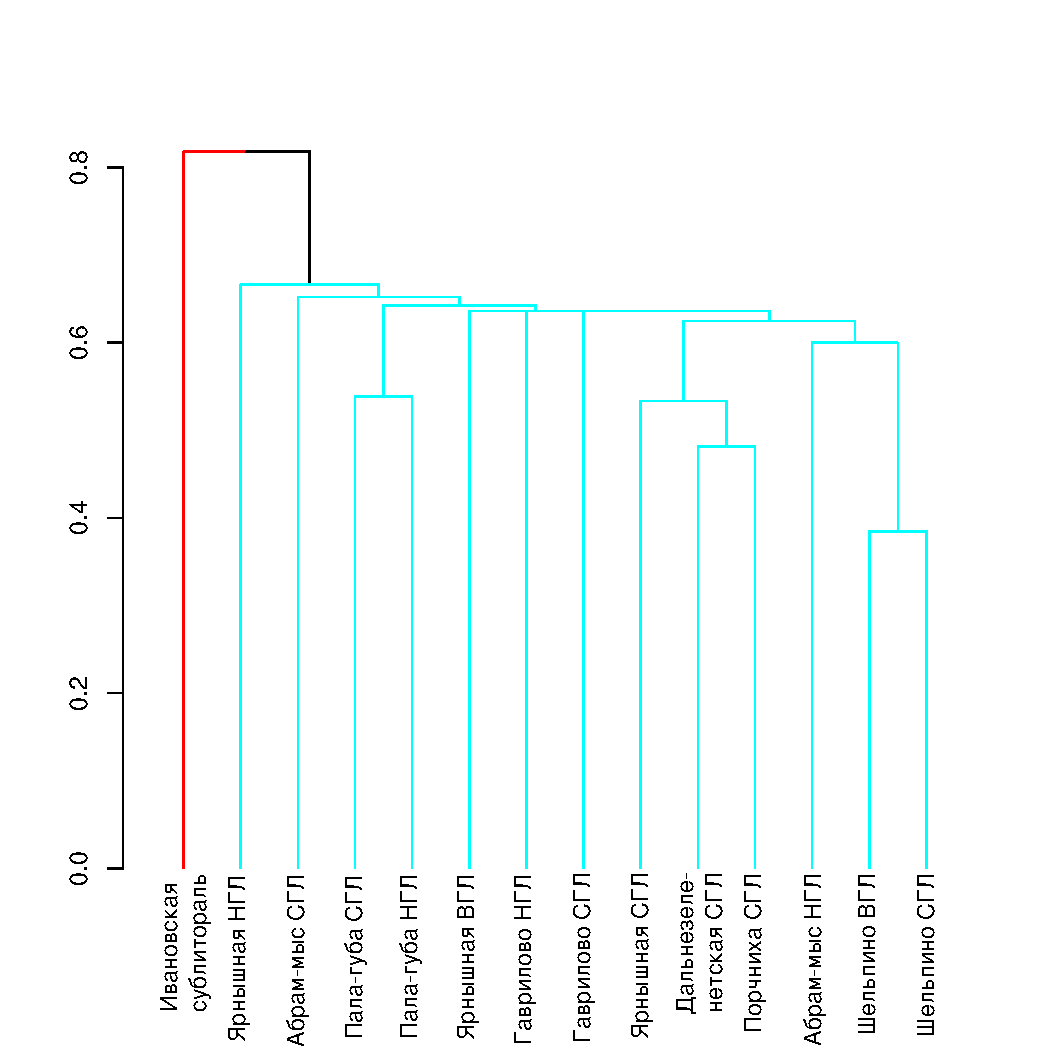
\includegraphics{../Barenc_Sea/soobshestvo/Barents_fauna_tidal_jaccard_single_1.pdf}
		\end{center}
	\caption{Классификация отдельных горизонтов литорали в Баренцевом море по видовому составу}
	\label{ris:cluster_barents_species_tidal}

	\footnotesize{Кластеризация по методу ближайшего соседа с использованием коэффициента Жаккара. По оси ординат --- коэффициент Жаккара. Цветом показаны кластеры, достоверно выделяющиеся при 5\% уровне значимости.}
	\end{figure}

Возможно, что была выбрана слишком дробная единица анализа, и посмотрим как распределятся полные описания сообществ по изученных участкам литорали (рис.~\ref{ris:cluster_barents_species_sites}. 
	\begin{figure}[p]
		\begin{center}
			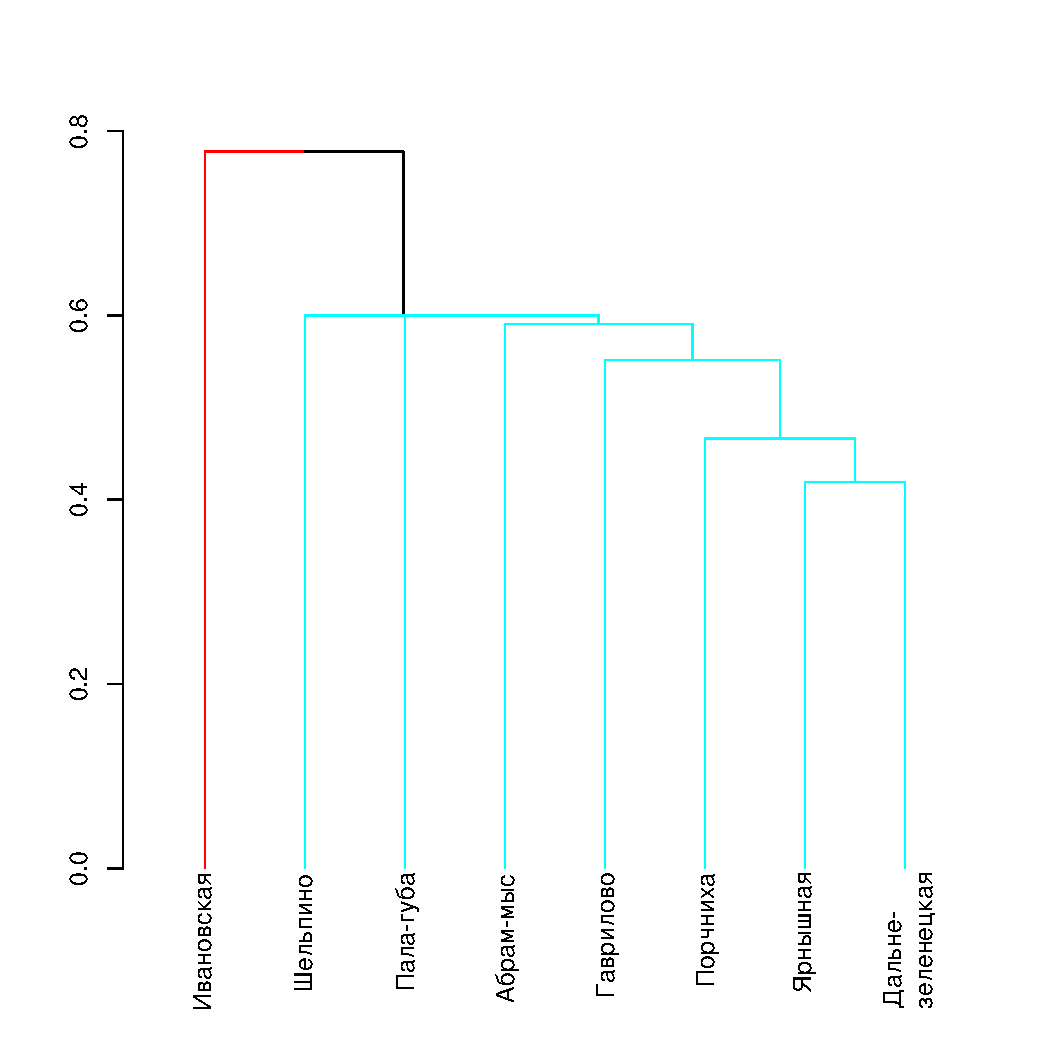
\includegraphics{../Barenc_Sea/soobshestvo/Barents_fauna_sites_jaccard_single_1.pdf}
		\end{center}
	\caption{Классификация исследованных участков в Баренцевом море по видовому составу}
	\label{ris:cluster_barents_species_sites}

	\footnotesize{Кластеризация по методу ближайшего соседа с использованием коэффициента Жаккара. По оси ординат --- коэффициент Жаккара. Цветом показаны кластеры, достоверно выделяющиеся при 5\% уровне значимости.}
	\end{figure}
Результат аналогичен, достоверно отличается только фауна губы Ивановская.


Для оценки влияния гранулометрического состава грунта на состав сообщества были выделены группы илисто-песчаная, песчаная и гравийно-песчаная литораль. 
В результате не было обнаружено достоверного влияния данного показателя на видовой состав сообщества ($R=0,053, p=0,36$).
	
Таким образом, таксономический состав сообществ на исследованных участках достаточно вариабелен, и по-видимому, сходство определяется географической близостью участков. 

%была еще тема на конференции в Мурманске. Не надо ли добавить оттуда и пересчитать все нафиг.

\subsection{Структура сообщества на литорали губы Дальне-Зеленецкая}
На литоральной отмели Дальний Пляж губы Дальне-Зеленецкой были проведены мониторинговые наблюдения за структурой сообщества.
В результате кластерного анализа по матрице коэффициентов Брей-Кертиса было выделено две достоверных (SIMPROF: p=0,05) группы (рис~\ref{ris:DZ_cluster_soobshestva}). 
	\begin{figure}[p]
		\begin{center}
			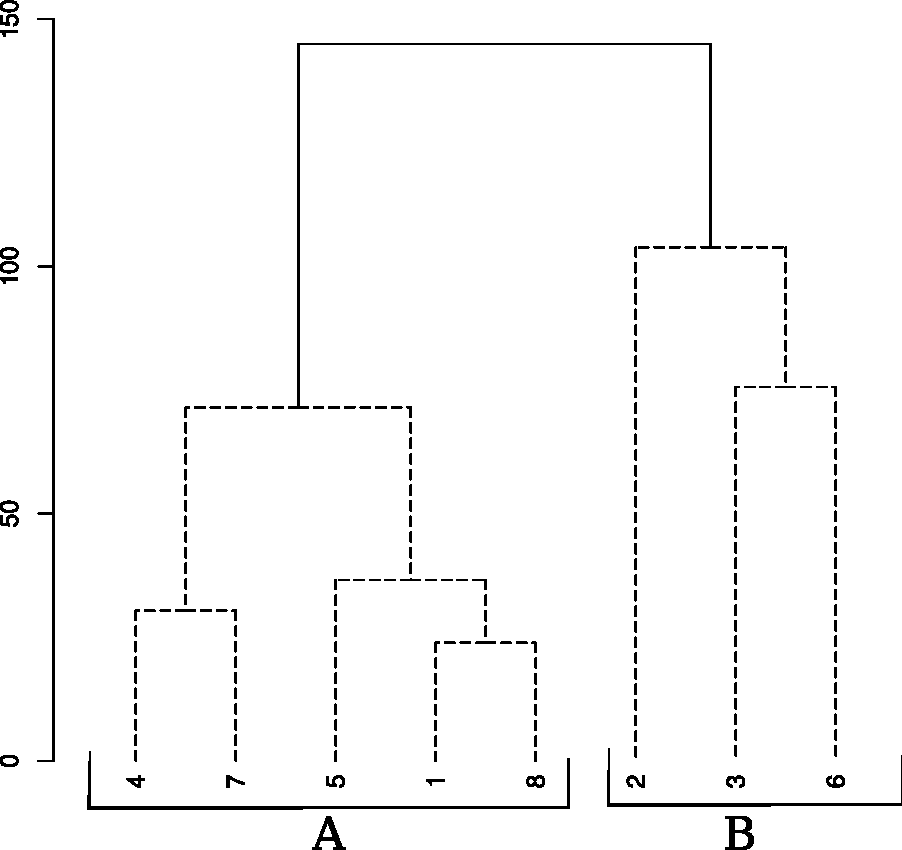
\includegraphics{../after_Deryuginskie/2_disser/station_bray_2002_SIMPROF_BW1.pdf}
		\end{center}
	\caption{Классификация станций на Дальнем пляже губы Дальнезеленецкая}
	\label{ris:DZ_cluster_soobshestva}

	\footnotesize{По оси ординат --- коэффициент Брея-Кертиса. Сплошными линиями показаны группы, достоверно выделяющиеся при 5\% уровне значимости.}
	\end{figure}

Сравнение двух выделенных зон по обилию видов-эдификаторов (рис.~\ref{ris:DZ_edifikatory}, A) показало что внутри выделенных групп станций их обилие различается. В группе А обилие полихет-трубкостроителей \textit{F.~sabella} максимально, и это подтверждает наше предположение, что эта группа соответствует сообществу полихет-трубкостроителей по терминологии Матвеевой с соавторами (\cite{Matveeva_et_al_1955}). 
	\begin{figure}[p]
	\begin{minipage}[b]{.46\linewidth}
	\begin{center}
	{\footnotesize А.{\it Fabricia sabella}}
		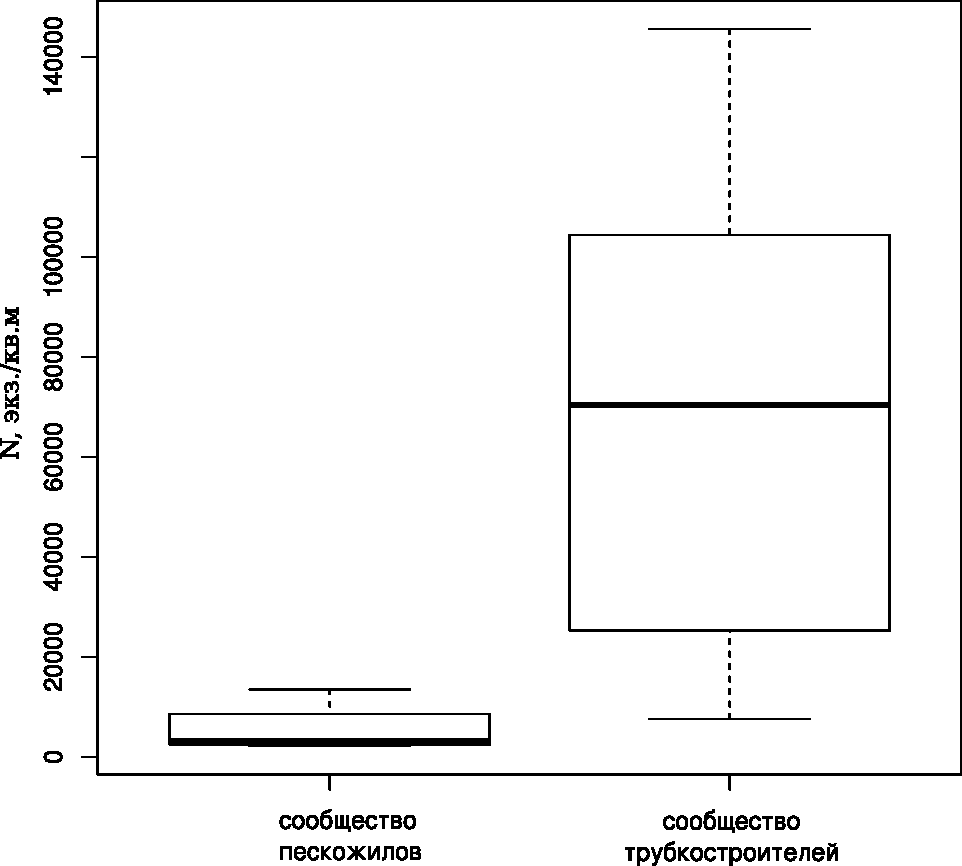
\includegraphics[width=\linewidth]{../after_Deryuginskie/2_disser/Fabricia_in_zones1.pdf}
	\end{center}
	\end{minipage}
	%
	\hfil %Это пружинка отодвигающая рисунки друг от друга
	%
	\begin{minipage}[b]{.46\linewidth}
	\begin{center}
	{\footnotesize Б. {\it Arenicola marina}}
		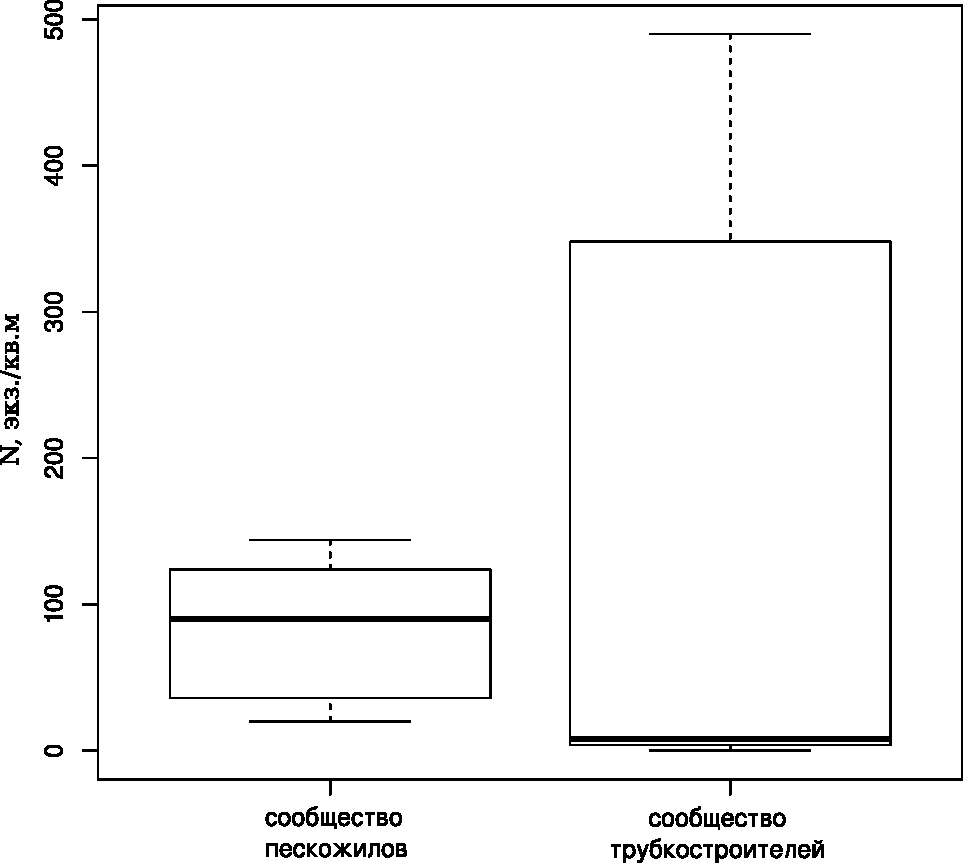
\includegraphics[width=\linewidth]{../after_Deryuginskie/2_disser/Arenicola_in_zones1.pdf}
	\end{center}
	\end{minipage}
	\caption{Обилие видов-эдификаторов в выделенных сообществах}
	{\footnotesize На графике: жирная горизонтальная линия --- медиана, границы <<ящика>> --- 1 и 3 квартили, <<усы>> --- $1,5$ интерквартильного расстояния, точки - значения выпадающие за $1,5$ интерквартильных расстояния}
	\label{ris:DZ_edifikatory}
	\end{figure}
Аналогично, среднее обилие пескожилов  \textit{A.~marina} в группе В на порядок превышает таковое в группе А (рис.~\ref{ris:DZ_edifikatory}, Б), и, несмотря на разнородность станций данной группы, можно говорить о их принадлежности к сообществу пескожилов по терминологии Матвеевой с соавторами.
Характерно, что два вида-эдификатора~--- \textit{Arenicola marina} и \textit{Fabricia sabella}~--- демонстрируют антагонизм в распределении на литорали.

Рассмотрим динамику массовых видов и доминантов на литорали Дальнего пляжа губы Дальне-Зеленецкой. 
Данные $1973$~года приведены по работе \cite{Agarova_et_al_1976}

\paragraph{\textit{Fabricia sabella}}
В течение исследованного периода средние значения плотности поселений {\it Fabricia sabella} находились в диапазоне от 5500~(32\%) до 169~тыс.~(10\%)~экз./м$^2$ в сообществе пескожилов и от 95~тыс.~(30\%) до 190~тыс.~(18\%)~~экз./м$^2$ для сообщества трубкостроителей (приложение~\ref{app:DZ_soobshestvo_dynamic}, рис.~\ref{ris:DZ_N_dynamic_dominants}). 
Однако изменения численности \textit{F.~sabella} были статистически недостоверны в обоих исследованных сообществах (табл.~\ref{tab:DZ_trends_Kruskal-Wallis}). 
\begin{table}[p]
\caption{Изменения плотности поселений массовых видов в исследованных сообществах на литорали г.~Дальне-Зеленецкая}
\label{tab:DZ_trends_Kruskal-Wallis}
\begin{tabularx}{\textwidth}{l|XXl|XXl}
\hline
сообщество: & \multicolumn{3}{c|}{трубкостроителей}&\multicolumn{3}{c|}{пескожилов}\\ \hline
                   & W               & p      &    & W         & p         &     \\ \hline
{\it Fabricia sabella}   & 7,5             & 0,11   &    & 6,2       & 0,18      &     \\
{\it Pygospio elegans}   & 15,2            & 0,0095 & ** & 2,2       & 0,82      &     \\
{\it Capitella capitata} & 16,5            & 0,0055 & ** & 20,8      & 0,0008    & *** \\
{\it Arenicola marina}   & 3,5             & 0,48   &    & 32,5      & 1.544e-06 & *** \\
{\it Oligochaeta}        & 9,3             & 0,0054 & ** & 5         & 0,28      &  	\\ \hline  
\end{tabularx}

{\footnotesize Примечание: W~--- значение критерия Краскела-Уоллеса, p~--- доверительная вероятность.}
\end{table}

По-видимому, это связано со значительным варьированием численности червей в отдельных пробах. 
Современная численность Fabricia sabella в сообществе пескожилов сравнима с обилием данного вида в 1973 году, но достоверно уменьшилась в сообществе трубкостроителей (табл.~\ref{tab:DZ_donimamnts_1973_2000}).
\begin{table}[p]
\caption{Сравнение плотностей поселения массовых видов на литорали Дальнего Пляжа г.~Дальне-Зеленецкой в 1973 и 2000-х годах.}
\label{tab:DZ_donimamnts_1973_2000}
\begin{tabularx}{\textwidth}{XX|X|XXX|X}
\hline
		 &		    & $1973$ год	      & \multicolumn {3}{c|}{2002-2007} &	различие    \\
вид              & сообщество       & $M$               & $Me$         & $2,5$\% $Q$ & $97,5$\% $Q$ & ($p < 0,05$) \\ \hline
{\it Fabricia sabella} & труб\-ко\-стро\-ите\-лей & 240000          & 99470      & 8538    & 217327   & есть                      \\
{\it Fabricia sabella} & пес\-ко\-жи\-лов       & 40000           & 19845      & 368     & 223808   & нет                       \\
{\it Pygospio elegans} & пес\-ко\-жи\-лов       & 20100           & 21805      & 838     & 101834   & нет                       \\
{\it Arenicola marina} & труб\-ко\-стро\-ите\-лей & 4               & 8          & 0       & 405,8    & нет                       \\
Oligochaeta      & пес\-ко\-жи\-лов       & 25000           & 24990      & 451     & 92793    & нет                       \\ \hline
\end{tabularx}

{\footnotesize Примечание: $M$~--- средняя плотность поселения, экз./м$^2$, $Me$~--- медианная плотность поселения, экз./м$^2$ $Q$~--- квантили распределения}
\end{table}

\paragraph{\textit{Pygospio elegans}} 
Средняя численность многощетинковых червей {\it Pygospio elegans} в разные годы была оценена в 27~(23\%)-36~(41\%)~тыс.~экз./м$^2$ в сообществе пескожилов и от 1800~(15\%)~экз./м$^2$ до 18~(36\%)~тыс.~экз./м$^2$ в сообществе трубкостроителей (приложение~\ref{app:DZ_soobshestvo_dynamic}, рис.~\ref{ris:DZ_N_dynamic_dominants}). 
В сообществе пескожилов обилие данного вида оставалось стабильным в течение всего периода наблюдений (табл.~\ref{tab:DZ_trends_Kruskal-Wallis}) и не отличалось от такового в 1973 году (табл.~\ref{tab:DZ_donimamnts_1973_2000}). 
В сообществе трубкостроителей наблюдались его достоверные колебания (табл.~\ref{tab:DZ_trends_Kruskal-Wallis}). 
В 2003 году численность данных червей была минимальна, после чего происходило ее плавное увеличение и к 2007 году она становилась сравнима со значением численности, отмеченным для 1973 года (приложение~\ref{app:DZ_soobshestvo_dynamic}, рис.~\ref{ris:DZ_N_dynamic_dominants}). 

\paragraph{\textit{Capitella capitata}}
Средняя численность {\it Capitella capitata} достоверно изменялась в течение исследованного периода (табл.~\ref{tab:DZ_trends_Kruskal-Wallis}). 
Максимальное обилие для обоих сообществ было отмечено в 2002 году (600~(62\%) в сообществе пескожилов и 1800~(71\%)~экз./м$^2$ в сообществе трубкостроителей), после чего до 2006 года были колебания, и в 2006 -- 2007 наметилось некоторое его увеличение (приложение~\ref{app:DZ_soobshestvo_dynamic}, рис.~\ref{ris:DZ_N_dynamic_dominants}). 
Численности, указанные для данного вида в 1973 году на порядок превышают  максимальные значения, полученные нами в исследованный период.

\paragraph{\textit{Arenicola marina}}
Средняя численность пескожилов в сообществе трубкостроителей была стабильно низкой (табл.~\ref{tab:DZ_trends_Kruskal-Wallis}) и не превышала 10~экз./м$^2$. 
В 1973 году численность не отличалась от современного уровня (табл.~\ref{tab:DZ_donimamnts_1973_2000}). 
В сообществе пескожилов численность титульного вида демонстрировала достоверные колебания (табл.~\ref{tab:DZ_trends_Kruskal-Wallis}), но во все годы была более 40~экз./м$^2$ (приложение~\ref{app:DZ_soobshestvo_dynamic}, рис.~\ref{ris:DZ_N_dynamic_dominants}). 
Максимальное обилие Arenicola marina здесь было отмечено в 2002 году (84~(14\%)~экз./м$^2$). 
Подобные численности были отмечены и в 1973 году (приложение~\ref{app:DZ_soobshestvo_dynamic}, рис.~\ref{ris:DZ_N_dynamic_dominants}).

\paragraph{\textit{Oligochaeta}}
Средняя численность Oligochaeta в течение исследованного периода находилась в диапазоне от 3~(46\%) до 38~(43\%)~тыс.~экз./м$^2$ в сообществе пескожилов и от 32~(54\%) до 106~тыс.~экз./м$^2$ в сообществе трубкостроителей (приложение~\ref{app:DZ_soobshestvo_dynamic}, рис.~\ref{ris:DZ_N_dynamic_dominants}). 
Обилие малощетинковых червей было стабильно в сообществе пескожилов и сравнимо со значениями обилия в 1973 году (табл.~\ref{tab:DZ_donimamnts_1973_2000}), но достоверно изменялось в сообществе трубкостроителей (табл.~\ref{tab:DZ_trends_Kruskal-Wallis}) за счет значительного его варьирования между отдельными пробами.

\medskip

Нами были проведены детальные исследования поселений инфаунных двустворчатых моллюсков, обитающих совместно с {\it Macoma balthica}: {\it Cerastoderma edule} и {\it Mya arenaria}. 
В связи с низкой встречаемостью моллюсков в пробах и низкой численностью мы проводили описание поселения в пределах всего Пляжа, без разделения на зоны.

Поскольку по методике сборов в 1970х годах пробы для учета моллюсков промывали на сите с диаметром ячеи $5$~мм, для сравнения мы корректировали наши данные с учетом размерной структуры и отдельно приводим численность особей крупнее $5$~мм.

\paragraph{\textit{Cerastoderma edule}}
Средняя численность {\it Cerastoderma edule} не превышала 25 экз./м2 (рис.~\ref{ris:DZ_N_dynamic_bivalve}). 
%
	\begin{figure}[p]
	
	\begin{minipage}[b]{.46\linewidth}
	\begin{center}
	{\footnotesize \textit{Cerastoderma edule}}
		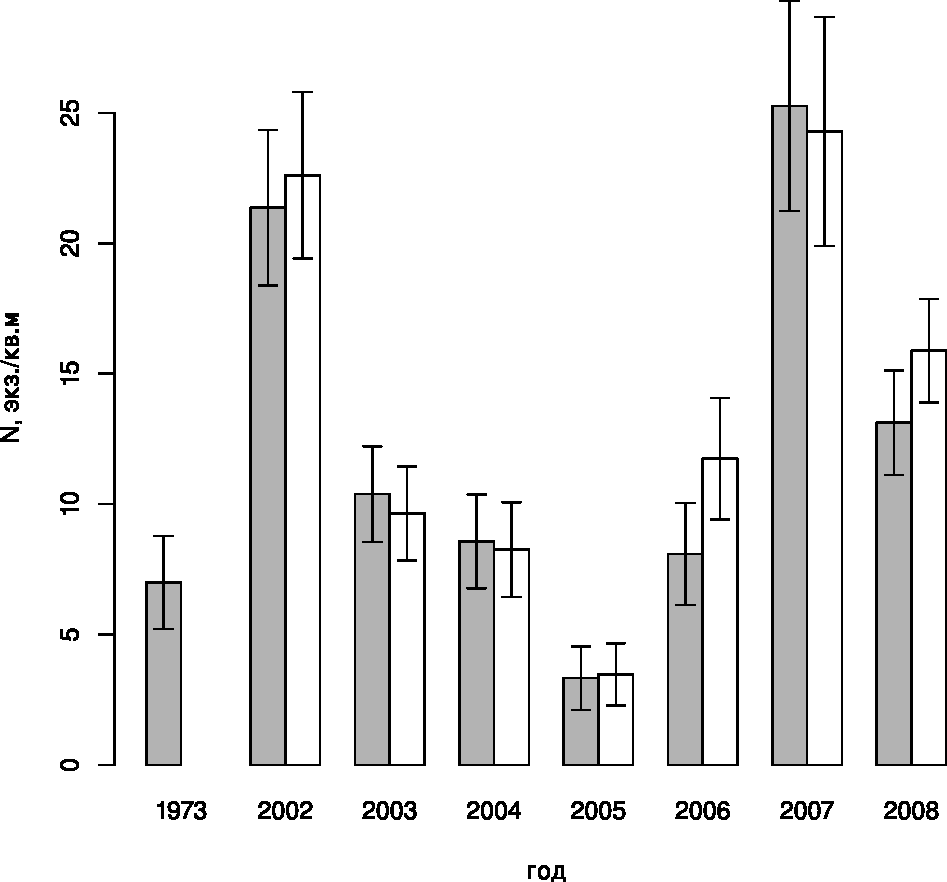
\includegraphics[width=55mm]{../after_Deryuginskie/2_disser/cockle_N_dynamic_all1.pdf}
	\end{center}
	\end{minipage}
	%
	\hfil %Это пружинка отодвигающая рисунки друг от друга
	%
	\begin{minipage}[b]{.46\linewidth}
	\begin{center}
	{\footnotesize \textit{Mya arenaria}}\\
		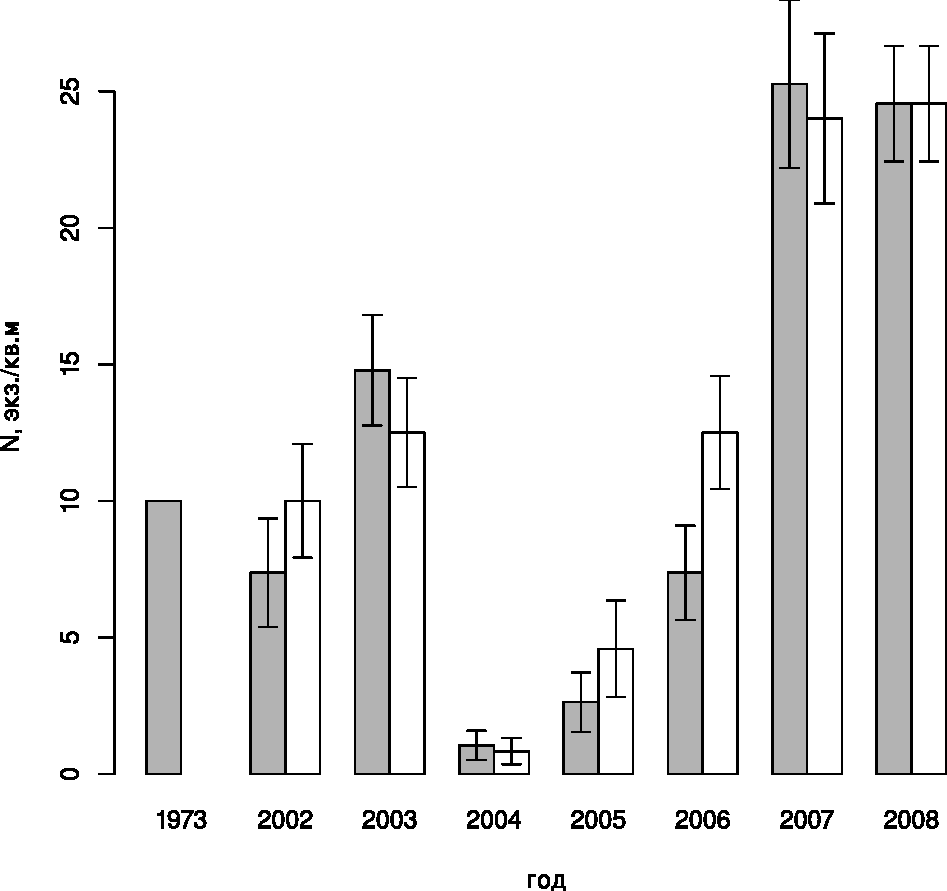
\includegraphics[width=55mm]{../after_Deryuginskie/2_disser/Mya_N_dynamic_all1.pdf}
	\end{center}
	\end{minipage}
\caption{Динамика обилия инфаунных моллюсков, обитающих совместно с {\it Macoma balthica}, на литорали Дальнего пляжа губы Дальне-Зеленецкой}
\label{ris:DZ_N_dynamic_bivalve}

{\footnotesize Примечание: N~--- плотность поселения, экз./м$^2$: белые столбцы~--- всех особей, серые столбцы~--- особей крупнее $5$~мм.}
\end{figure}
%
За все годы наблюдения плотность поселения сердцевидки достоверно изменялась (тест Краскел-Уоллиса: $W=16,2, p=0,01$), и было отмечено $2$ локальных максимума: в $2002$ и в $2007$~годах. 
Минимальное обилие было отмечено в $2005$~году. 
Количество моллюсков с длиной раковины более $5$~мм в период низкой численности (2004-2006 гг.) было сравнимо с плотностью поселения в 1973 году.

В разные годы минимальный размер особей Cerastoderma edule в пробах колебался от $2$ до $7$~мм (рис.~\ref{ris:DZ_size_str_bivalve}). 
%
	\begin{figure}[p]
		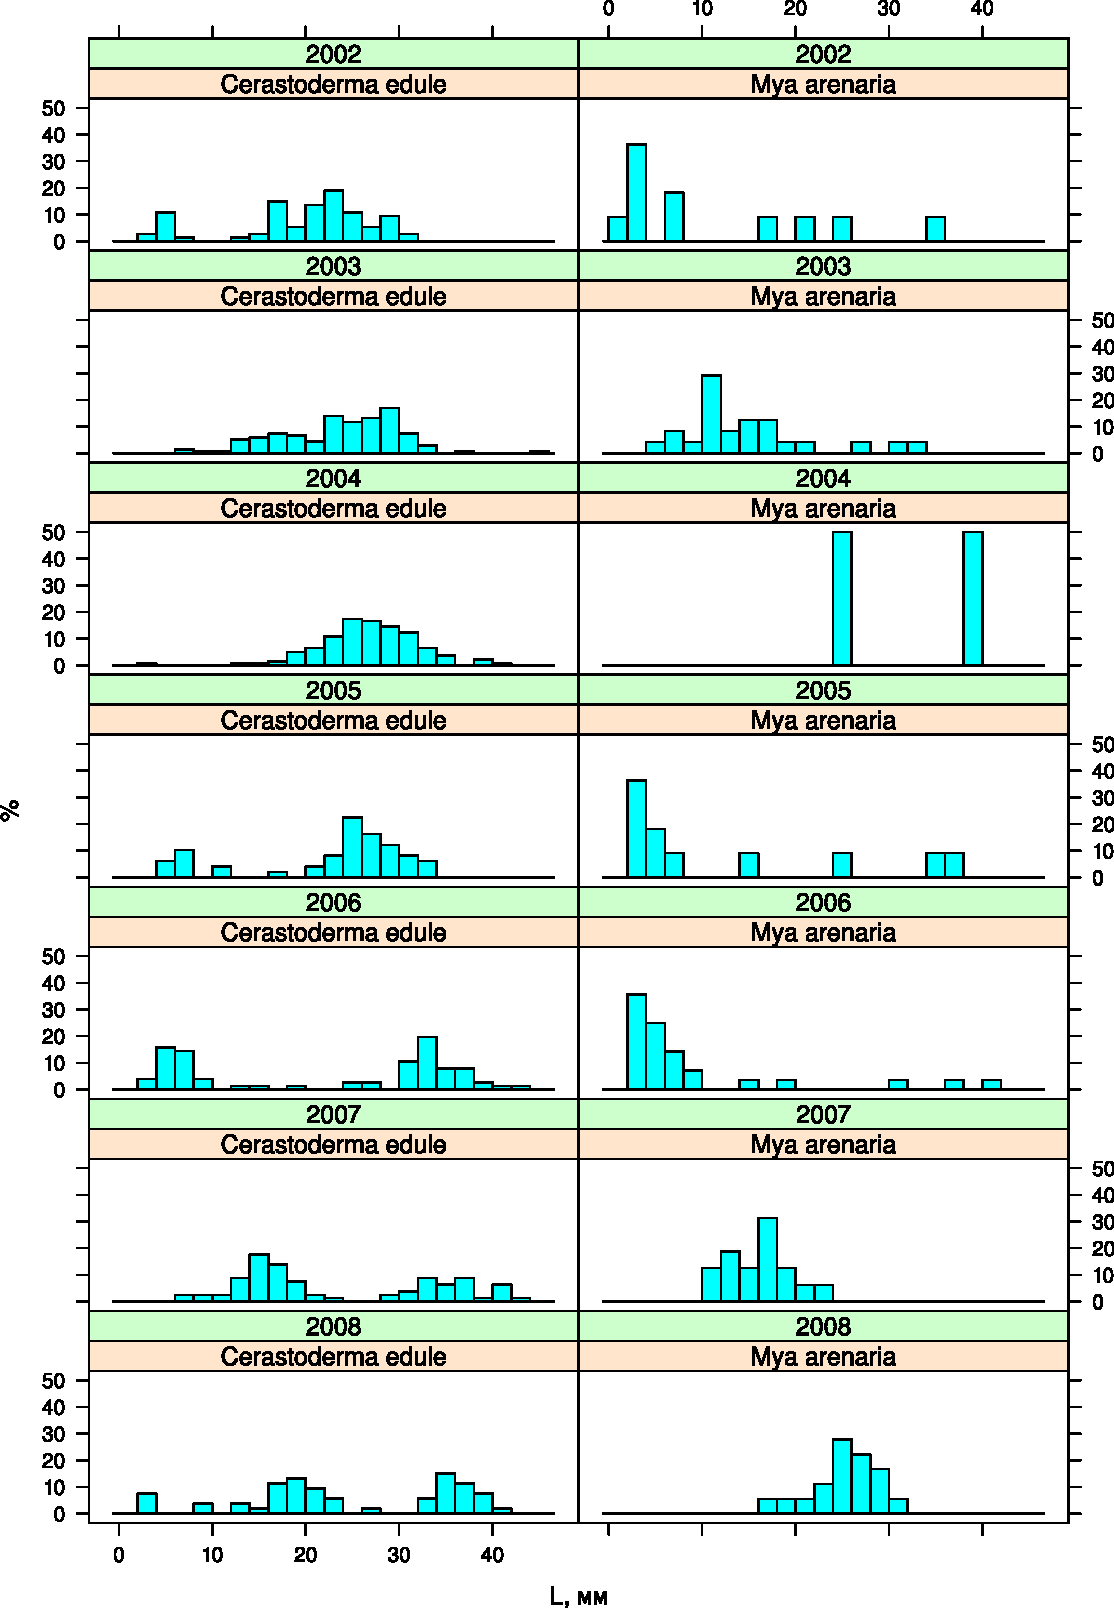
\includegraphics[height=.9\textheight]{../after_Deryuginskie/2_disser/size_structure_Cerastoderma_Mya_2mmclass1.pdf}
\caption{Размерная структура инфаунных моллюсков, обитающих совместно с {\it Macoma balthica}, на литорали Дальнего пляжа губы Дальне-Зеленецкой}
\label{ris:DZ_size_str_bivalve}

{\footnotesize Примечание: L,~мм~--- длина раковины, по оси ординат указана доля особей с соответствующей длиной раковины в сборах}
\end{figure}
%
Для данного региона это соответствует возрасту $1-2$ года (\cite{Genelt-Yanovskiy_et_al_2010}). 
Таким образом, пополнение молодью происходит не ежегодно. 
Максимальный размер особей в разные годы колебался от $32$ до $45$~мм. 
Годы снижения численности (2003 -- 2005) характеризовались практически полным отсутствием мелких особей. 
В то же время, максимальной плотности поселения сердцевидок ($2007$ год) совпал максимальным обилием некрупных особей ($7 - 21$~мм). 
Таким образом, характер динамики определяется массовостью пополнения поселения молодью.

\paragraph{\textit{Mya arenaria}}
Плотность поселения {\it Mya arenaria} за исследованные годы не превышала 25~экз./м$^2$ (рис.~\ref{ris:DZ_N_dynamic_bivalve}). 
Отмеченные колебания были статистически достоверны (тест Краскел-Уоллиса: $W=38,4, p<0,0001$).  
После относительно стабильного периода 2002 -- 2003 годов произошло резкое уменьшение плотности поселения мий в 2004 году, после чего она медленно увеличивается в период до 2006 года. 
В 2007 -- 2008 годах происходит резкое увеличение плотности поселения мий до максимальных значений за весь период наблюдений.
По характеру динамики размерной структуры можно предположить, что в 2002 -- 2003 году мы наблюдаем одну генерацию моллюсков, которая практически полностью элиминируется к 2004 году (рис~\ref{ris:DZ_size_str_bivalve}). 
В 2006-2008 году мы наблюдаем следующую генерацию, по-видимому, 2004 или 2005 года оседания.

\afterpage{\clearpage}
